\documentclass[12pt]{article}
\usepackage{fullpage}
\usepackage{graphicx}
\usepackage{sidecap}
\usepackage{algorithmic}
\usepackage{algorithm2e}
\usepackage{bbm}
\usepackage{amssymb}
\usepackage{amsmath}
\usepackage{amsfonts}
\usepackage{amsthm}
\usepackage{yhmath}
\usepackage{siunitx}
\usepackage[mathscr]{euscript}
\usepackage{enumerate}
\usepackage{mathtools}
\usepackage[hmargin=1in,vmargin=1in]{geometry}
\usepackage{graphicx}
\usepackage{subfigure}
\usepackage{setspace}
\usepackage{systeme}
\linespread{1.4142}
\graphicspath{ {./images/} }

\newcommand{\Z}{\mathbb{Z}}
\newcommand{\Q}{\mathbb{Q}}
\newcommand{\R}{\mathbb{R}}
\newcommand{\C}{\mathbb{C}}
\newcommand{\curve}{\mathcal{C}}
\newcommand{\integral}{\int\limits}


\begin{document}
\begin{figure}[!htbp]
    \centering
    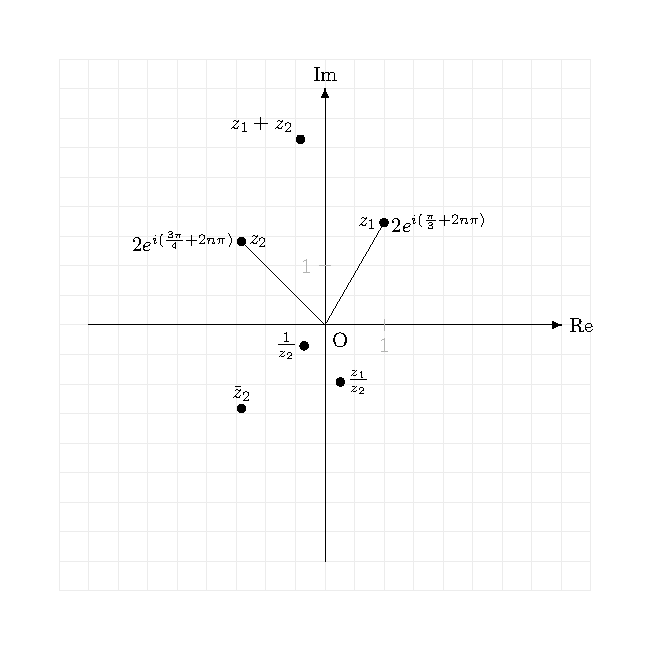
\includegraphics[width=1 \linewidth]{test1.pdf}
    \caption{$\C$}
\end{figure}

\begin{enumerate}
    \item $z_1 = 1 + i\sqrt3$ and $z_2 = -\sqrt2 + i\sqrt2$
    \begin{enumerate}
        \item Plotting $z_1$ and $z_2$ into the plane
        \item $z_1+z_2 = (1-\sqrt2) + i(\sqrt2 + \sqrt3)$
        \item $\bar z_2 = -\sqrt2 -i\sqrt2$
        \item $\frac{1}{z_2} = \frac{\bar z_2}{|z_2|} = \frac{-\sqrt2 - i\sqrt2}{4}$
        \item $z_1 = 2\exp(i(\frac{\pi}{3} + 2n\pi))$ and $z_2 = 2 \exp(i(\frac{3\pi}{4} + 2n\pi))$ for $n \in \mathbb{N}$
        \item $\frac{z_1}{z_2} = \frac{1+i\sqrt3}{-\sqrt2 + i\sqrt2} = \frac{(1+i\sqrt3)(-\sqrt2 - i\sqrt2)}{4} = \frac{( \sqrt6 - \sqrt2) -i(\sqrt2 + \sqrt6)}{4}$
    \end{enumerate}

    \item $z = \sqrt3 - i = 2\exp(i(\frac{7\pi}{6} + 2n\pi))$ for $n \in \mathbb{N}$, so the three roots of $z$ are
    \begin{itemize}
        \item $c_0 = \sqrt[3]2 \exp(i(\frac{7\pi}{18}))$
        \item $c_1 =  \sqrt[3]2 \exp(i(\frac{7\pi}{18} + \frac{2\pi}{3}))$
        \item $c_2 =  \sqrt[3]2 \exp(i(\frac{7\pi}{18} + \frac{4\pi}{3}))$
    \end{itemize}

    \item
    $|Im (z^2 + 2\bar z +3)| \le |z^2 + 2\bar z +3| \le |z^2| + 2|\bar z| + 3 = |z|^2 + 2|z| + 3 \le 2^2 + 2\times2 + 3 = 11$

    \item
    \begin{enumerate}
        \item $f(re^{i\theta}) = u(r, \theta) + iv(r, \theta) = r^{-3}\cos(-3\theta) - ir^{-3}\sin(3\theta)$

        So, $u(r, \theta)  = r^{-3}\cos(-3\theta)$, and $v(r, \theta) = r^{-3}\sin(-3\theta)$.

        Taking the partial derivatives yields, $$r u_r = v_\theta = -3r^{-3}\cos(-3\theta)$$ and $$u_\theta = -r v_r = -3r^{-4}\sin(-3\theta)$$ which exists for all $r \not = 0$ and any $\theta$.

        So $f$ is differentiable on $\C \setminus \{0\}$ \\ and $f'(r, \theta) = e^{-i\theta}(u_r + iv_r) = -e^{-i\theta}(3r^{-4}\cos(-3\theta) + i3r^{-4}\sin(-3\theta))$.

        \item $f(z) = \sin(\bar z)$

        Consider, for $x\in\R$, $\cosh(x) = \frac{e^x + e^{-x}}{2}$, so $\cosh(x)' = \frac{e^x - e^{-x}}{2} = \sinh(x)$. Also, $\sinh(x) =  \frac{e^x - e^{-x}}{2}$, so $\sinh(x)' =  \frac{e^x + e^{-x}}{2} = \cosh(x)$.

        Also, $\sinh(x) = 0$ when $ x = 0$ and, for all $x\in\R$, $\cosh(x) \not = 0$.

        For $z = x+iy$,
        \begin{align*}
            f(z) = \sin(\bar z) &= \sin(x)\cosh(-y) + i\cos(x)\sinh(-y) \\
            &= \sin(x)\cosh(y) - i\cos(x)\sinh(y)
        \end{align*}

        The components are $u(x, y) = \sin(x)\cosh(y)$ and $v(x,y) = -\cos(x)\sinh(y)$.

        Taking the partial derivatives yields, $$u_x = - v_y = \cos(x)\cosh(y)$$ and $$v_x = u_y = \sin(x)\sinh(y)$$

        For the Cauchy-Riemann to be satisfied, both equations must equal to $0$. \\Since $\cosh(y)$ cannot be $0$, $\cos(x) = 0$. So $x = \frac{\pi}{2} + n\pi$ for $n \in \mathbb{N}$.
        When $x$ as above, $\sin(x) = 1$, so $\sinh(y) = 0$, or $y = 0$.

        So $f$ is differentiable in all real numbers $\frac{\pi}{2} + 2n\pi$ for $n \in \mathbb{N}$, \\and $f'(z) = u_x + iv_x = \cos(x)\cosh(y) + i\sin(x)\sinh(y)$.
    \end{enumerate}

    \item\begin{enumerate}
            \item The set $\C \setminus \{0\}$ is open, and $f$ has derivatives everywhere in that set, so $f$ is analytic on $\C \setminus \{0\}$.
            \item For any point described above, any neighborhoods around that point will contain some complex numbers, any of which $f$ does not have derivatives at. So $f$ is nowhere analytic in $\C$.
        \end{enumerate}

    \item The principal value of $(1+i\sqrt3)^{4i}$,
        \begin{align*}
            (1+i\sqrt3)^{4i} &= \exp(4i ~\text{Log}(1+i\sqrt3)) \\
            &= \exp\left(4i ~ \left(\ln(2) + i\frac{\pi}{3}\right)\right) \\
            &= \exp\left(-\frac{4\pi}{3} + i\ln(16)\right)\\
            &= \frac{\cos(\ln16)}{e^{\frac{4\pi}{3}}} + i\frac{\sin(\ln16)}{e^{\frac{4\pi}{3}}}
        \end{align*}
    \pagebreak
    \item The contour's parameterization: $z(t) =  2e^{it}$ for $\frac{\pi}{3} \le t \le \frac{3\pi}{4}$

    Then
    \begin{align*}
        \int_\curve 3z^2 - 2z + 1 dz &= \integral^\frac{3\pi}{4}_\frac{\pi}{3} f(z(t))z'(t)dt\\
        &= \integral^\frac{3\pi}{4}_\frac{\pi}{3} (12e^{2it} - 4e^{it} + 1)(2ie^{it}) dt \\
        &= \integral^\frac{3\pi}{4}_\frac{\pi}{3} 24ie^{3it} - 8ie^{2it} + 2ie^{it} dt\\
        &\left. = 8e^{3it} -4e^{2it} +2e^{it} \right\vert_{\frac{\pi}{3}}^{\frac{3\pi}{4}}\\
        &= 3\sqrt2 + 5+ i (5\sqrt2 + 4 + \sqrt3)
    \end{align*}

    \item
    \begin{enumerate}
        \item $f(z) = \log z$, and the parameterization $z(t) = 2e^{it}$ for $\frac{\pi}{2} < t < \frac{5\pi}{2}$.

        Consider $f(z(t)) = \log(2e^{it}) = \ln2 + it$, so
        \begin{align*}
        f(z(t)) z'(t) &= (\ln2 +it)2ie^{it}\\
        &= 2i(\ln2 + it)(\cos t + i\sin t)\\
        &= (-2t\cos t - \ln4 \sin t )+ i(\ln4 \cos t - 2t\sin t)
        \end{align*}

        Since  $\lim\limits_{t \to \frac{\pi}{2}^{+}} f(z(t))z'(t)$ exists and equals to $-\ln4 - i\pi$,
        it is piecewise continuous on $[\frac{\pi}{2}, \frac{5\pi}{2}]$ and the integral exists.

        Finally,
        \begin{align*}
            \int_\curve f(z)dz &= \integral^{\frac{5\pi}{2}}_{\frac{\pi}{2}}  (-2t\cos t - \ln4 \sin t )+ i(\ln4 \cos t - 2t\sin t) dt\\
            & =\left. -2t\sin t -2\cos t + \ln4 \cos t + i (\ln4 \sin t + 2t\cos t - 2\sin t) \right\vert ^{\frac{5\pi}{2}}_{\frac{\pi}{2}}\\
            &= -4\pi
        \end{align*}
        \pagebreak
        \item $e^z-2z+ 1$ is the sum of three entire functions, so it is entire. \\So $\int_\curve f(z)dz = 0$ by Cauchy-Goursat Theorem.
        \item \begin{align*}
        \int_\curve \frac{z+1}{z^2-3z}dz &= \int_\curve \frac{1}{z} + \frac{4}{3} \left(\frac{1}{z-3} + \frac{1}{z}\right) dz \\
        &= \int_\curve \frac{1}{z}dz + \frac{4}{3} \int_\curve \frac{1}{z-3} dz + \frac{4}{3}\int_\curve \frac{1}{z} dz\\
        &= 2\pi i + \frac{4}{3} \times 0 + \frac{4}{3} 2\pi i \\
        &= \frac{14}{3} \pi i
        \end{align*}

        The first and third integral is due to Cauchy's integral formula, and the second is due to Cauchy-Goursat theorem.

    \item $z^3- i$ is a polynomial, thus is entire. Then, by Cauchy's integral formula,  $$\int_\curve \frac{z^3-i}{(z-i)^3}dz = \frac{2\pi i}{2!}\times (z^3 - i)''(i) = -6\pi$$
    \end{enumerate}

\end{enumerate}

\end{document}

\begin{comment}

to delete files: latexmk -c

to compile: pdflatex (filename).tex

to add a pdf
\begin{figure}[!htbp]
    \centering
    \includegraphics[width=1 \linewidth]{{filename}.pdf}
    \caption{Data sheet}
\end{figure}

\end{comment}
